% !TEX root = ../main.tex
\title{Multi-Subject \acrlong*{pfm}}
\label{cha:multi-subject}

\begin{framed}\noindent This chapter is in preparation to be published and will
    be available as an interactive website
    \url{https://github.com/eurunuela/msPFM\_paper}.
\end{framed}

Functional magnetic resonance imaging (fMRI) during naturalistic paradigms has
become increasingly popular in cognitive neuroscience as a way to investigate
cognition and behaviour within more ecologically valid contexts. However,
current methods for fMRI data analysis in naturalistic paradigms are limited in
how they can characterize the precise spatio-temporal dynamics of neural
activity evoked by naturalistic stimuli. On the one hand, model-based
approaches, such as traditional general linear model (GLM) analyses and encoding
models, make strong assumptions about what features of the stimulus might be
important and when they ocurr, which limits an accurate interpretation of the
resulting maps of blood oxygenation-level dependent (BOLD) activity. On the
other hand, model-free approaches, such as inter-subject correlation and event
segmentation algorithms, make no assumptions about stimulus features, but
necessitate combining information across multiple time points, making it
difficult to trace the recovered signal back to particular moments in the
stimulus. To address these limitations, this chapter introduces a novel method
for fMRI data analysis in naturalistic paradigms, called multi-subject
\acrlong*{pfm} (msPFM). Unlike existing approaches, msPFM estimates shared and
individualized neuronal-related brain responses at the finest spatial and
temporal resolution available in fMRI data. The msPFM algorithm implements a
multivariate regularized least-squares algorithm for hemodynamic deconvolution
of fMRI data that estimates the neuronal-related BOLD activity without relying
on the temporal structure of the stimuli. Its performance is demonstrated
through simulations and experimental movie-watching datasets, showcasing its
ability to detect moment-to-moment neuronal-related activity patterns associated
with low- and mid-level features of the movie. Furthermore, msPFM reveals a
spatial cortical gradient of BOLD activity that aligns with previous findings
obtained with event segmentation methods. It also provides an extra temporal
dimension to the maps obtained with intersubject correlation analyses.  
In summary, msPFM offers a powerful tool for exploring the spatio-temporal 
dynamics of the rich patterns of neural activity evoked by naturalistic fMRI paradigms. 
Researchers can access the open-source Python package for msPFM at
\url{https://github.com/ParadigmFreeMapping/msPFM}.

\section{Introduction}
\label{sec:multi_subject_introduction}

The use of movies and stories in the so-called naturalistic paradigms combined
with functional magnetic resonance imaging (fMRI) has increased considerably in
recent years as a replacement for task and resting state experimental paradigms
to study human cognition and mapping brain function \citep{Finn2021Isittime}. It
owes its popularity not only to its similarity with freeform cognition and
unconstrained behaviour, but also to the fact that individual differences in
functional connectivity are more stable
\citep{Vanderwal2017Individualdifferencesfunctional,
Wang2017Testretestreliability} and offer improved predictions of behavior
\citep{Finn2021Moviewatchingoutperforms}. Furthermore, naturalistic paradigms
have emerged as valuable tools for investigating various neurological and
developmental disorders. For example, studies utilizing movie-watching have
revealed distinct functional network configurations among individuals with
autism, highlighting their idiosyncratic patterns
\citep{Bolton2018BraindynamicsASD,Bolton2020Neuralresponsesautism}.
Additionally, research has demonstrated a reduction in intersubject correlations
within attention-related brain areas among individuals with attention deficit
hyperactivity disorder (ADHD), indicating a desynchronization of brain activity
in this diseased population \citep{Salmi2020ADHDdesynchronizesbrain}.
Movie-watching fMRI has also been utilized to investigate the memory
representations of healthy individuals during the retrieval of movie scenes,
which revealed a shared spatial organization among subjects exposed to identical
naturalistic stimuli \citep{Chen2017Sharedmemoriesreveal}. Finally, naturalistic
paradigms have played a crucial role in demonstrating the meaningful structure
and reliability of movie scene segmentation across subjects
\citep{Raccah2022Acousticfeaturesdrive, Speer2009ReadingStoriesActivates,
Zacks2009Usingmovementintentions}. Notably, studies have revealed that
variations in these patterns of event segmentation are associated with age,
cognitive abilities \citep{Bailey2017Attentionalfocusaffects,
Jafarpour2022Eventsegmentationreveals, Zacks2006Eventunderstandingmemory}, and
clinical conditions \citep{Zalla2004Perceptiondynamicaction}.

Several techniques have been employed to analyze naturalistic fMRI data. One
such technique is intersubject correlation (ISC), which involves calculating the
synchrony among the voxelwise signals of multiple subjects throughout the data
acquisition process
\citep{Hasson2004IntersubjectSynchronizationCortical,Wilson2007SuperiorTemporalCortex,Nastase2019Measuringsharedresponses,Jangraw2023Intersubjectcorrelation,Chen2020Untanglingrelatednesscorrelations}.
An extension to this approach incorporates the temporal dimension with the
sliding window ISC method (averaging ISC over a temporal window of a few
volumes) or the instantaneous phase synchronization
\citep{Glerean2012FunctionalMagneticResonance}, These approaches generate
voxelwise measures of moment-to-moment synchrony
\citep{Nummenmaa2012Emotionspromotesocial}, which can then be contrasted against
stimulus models, offering an intermediate approach that combines aspects of
stimulus-dependent and stimulus-free analyses. However, the degree of synchrony
is calculated during the entire acquisition or within the win dow duration, i.e.
spanning over multiple TRs. Intra and inter-subject correlation of functional
connectivity \citep{Vanderwal2017Individualdifferencesfunctional} and the
intersubject correlation of dynamic connectivity
\citep{Di2020Intersubjectconsistentdynamic} offer additional approaches for
investigating naturalistic fMRI data that examine the interplay between brain
regions and the consistent patterns of connectivity across individuals.
Alternatively, the detection of event segmentation boundaries has also been a
major focus in the development of data analysis techniques for naturalistic
paradigms. Currently, two main state-of-the-art techniques are mostly used to
blindly identify temporal boundaries within a sequence of events without prior
knowledge: hidden Markov models (HMM)
\citep{Baldassano2017DiscoveringEventStructure} and greedy state boundary search
(GSBS) \citep{Geerligs2021Detectingneuralstate}. Finally, another strategy
involves constructing encoding models that utilize representations extracted
from neural network language models to forecast BOLD responses to natural
language stimuli \citep{Jain2020Interpretablemultitimescale}, as well as the use
of deep neural network models using human visual areas to learn non-hierarchical
representations \citep{StYves2023Brainoptimizeddeep}.

However, the aforementioned methods have several limitations. First, ISC reveals
widespread synchronization across individuals without specific associations with
events of particular cognitive functions throughout a scan. Although
sliding-window ISC can enhance temporal resolution for characterizing such
events, it should be noted that this technique does not offer the utmost level
of temporal precision. Second, the HMM and GSBS operate at the ROI level, and
hence provide a low spatial resolution that does not allow the discovery of
precise, individualized spatial patterns. More importantly, all these techniques
summarize the within-region fMRI signal into states or connectivity patterns
that are sustained over several TRs, and therefore, they do not capture temporal
dynamics at the fastest temporal resolution available in the data, i.e., at the
\acrshort*{tr} level. In summary, these methods rule out the precision mapping
of idiosyncratic spatio-temporal patterns evoked by naturalistic stimuli. One
possible approach to address this issue is to employ data-driven techniques that
operate at the TR and voxel level. Hemodynamic deconvolution is a method that
falls under this category \citep{Gaudes2010Detectioncharacterizationsingle,
Karahanoglu2013TotalactivationfMRI,
Urunuela2023HemodynamicDeconvolutionDemystified}. It has the ability to estimate
neuronal-related activity without relying on the temporal information of the
experimental paradigm, and as a result, it proves to be particularly valuable
when dealing with naturalistic stimuli.

Here, we introduce a novel method for the analysis of naturalistic fMRI data
called multi-subject \acrlong*{pfm} (msPFM) that overcomes the limitations
mentioned above. msPFM solves a multivariate regularized least-squares problem
for hemodynamic deconvolution of the fMRI signal across subjects to blindly
estimate the shared and individualized neuronal-related activity without
requiring any temporal model of the stimulus. Unlike previous methods for
naturalistic fMRI data, this formulation allows the msPFM algorithm to operate
at the fastest temporal resolution (TR), and the highest spatial resolution
(voxel). We introduce msPFM and evaluate the method in simulations and two
experimental datasets with movie-watching paradigms to showcase its potential to
elucidate moment-to-moment spatio-temporal neural activity patterns evoked by
naturalistic paradigms and assess their ability to map low- and mid-level movie
features. The datasets, \textit{Iteration} and \textit{Sherlock}, differed in
terms of the studied low- and mid-level features, subject counts (43 vs 16), and
data type (multi-echo vs single-echo).

\section{Multi-subject \acrlong*{pfm}}

\subsection{Signal Model}

In gradient-echo fMRI acquisitions, the time series of a voxel $v$ normalized to
signal percentage change can be approximated with the following linear
relationship with the echo time (TE) \citep{Kundu2017MultiechofMRI}: 
\begin{equation}
    y(v,TE_k, t) \approx \Delta \rho(v,t) - TE_k \Delta
    R_2^*(v,t) + \epsilon(v,t),
\end{equation}
where $\Delta R_2^*(v,t)$ represents BOLD-like changes, $\Delta \rho(v,t)$
describes changes in the net magnetization, and $\epsilon(v,t)$ is a random
noise term. Changes in the net magnetization $\Delta \rho(v,t)$ are mostly due
to motion- and hardware-related artefacts, which can be reduced in preprocessing
by using denoising tools such as ICA-AROMA \citep{Pruim2015ICAAROMArobust} for
single-echo acquisitions or ME-ICA \citep{Kundu2012DifferentiatingBOLDnon,
Kundu2017MultiechofMRI} for multi-echo acquisitions. Hereinafter, the term
$\Delta \rho(v,t)$ can be neglected for a simpler notation. 

Following the same notation described in previous chapters, let us also consider
that changes in $R_2^*(v,t)$ that are related to neuronal activity will follow a
linear time-invariant model that is defined as the convolution of the
activity-inducing signal $s(v,t)$ with the hemodynamic response $h(v,t)$
\citep{Boynton1996LinearSystemsAnalysis,
Glover1999DeconvolutionImpulseResponse}. Considering the signal is sampled at
every TR, the previous signal model can be written in discrete matrix form as
$\mathbf{y}_{v} = -TE_ k \mathbf{H} \mathbf{s}_{v} + \boldsymbol{\epsilon}_{v}$,
where $\mathbf{H} \in \mathbb{R}^{N \times N}$ is the Toeplitz convolution
matrix with shifted versions of the hemodynamic response function (HRF)
\citep{Gitelman2003Modelingregionalpsychophysiologic,
Gaudes2013Paradigmfreemapping}, $\mathbf{y}_v$, $\mathbf{s}_v$,
$\boldsymbol{\epsilon}_{v} \in \mathbb{R}^{N}$, and $N$ is the number of scans
(i.e. TRs). 

Without loss of generalization, we assume that the HRF model is the same across
voxels. As described in \cref{cha:synthesis_analysis}, the activity-inducing
signal $\mathbf{s}_{v}$ can also be written in terms of the innovation signal
$\mathbf{u}_v$ as $\mathbf{s}_{v} = \mathbf{Lu}_{v}$, where the matrix
$\mathbf{L} \in \mathbb{R}^{N \times N}$ is the first-order integration operator
\citep{Cherkaoui2019Sparsitybasedblind,
Urunuela2020StabilityBasedSparse,Urunuela2023HemodynamicDeconvolutionDemystified}.
Hence, the signal model for a given $TE_k$ (i.e. single-echo) can be written as
follows:
\begin{equation}
\label{eq:signal_model_single_echo}
    \mathbf{y}_{v,k} = - TE_{k} \mathbf{HL} \mathbf{u}_{v} + \boldsymbol{\epsilon}_v,
\end{equation}
which can be extended for a multi-echo acquisition by concatenating the time
series of each echo ($k=1,\ldots,K$) in a single vector:
\begin{equation}
\label{eq:signal_model_multi_echo}
\left[\begin{array}{c} \mathbf{y}_{v,1} \\
    \vdots \\
    \mathbf{y}_{v,K} 
\end{array}\right]
=
\left[\begin{array}{c} -\mathrm{TE}_{1} \mathbf{HL} \\
    \vdots \\
    -\mathrm{TE}_{K} \mathbf{HL}
\end{array}\right]
\mathbf{u}_v
+
\left[\begin{array}{c} \boldsymbol{\epsilon}_{v,1} \\
    \vdots  \\
    \boldsymbol{\epsilon}_{v,K}
\end{array}\right].
\end{equation}

Assuming that data from multiple subjects ($s=1,\ldots,S$) are aligned to a
common space, the multivariate multi-echo formulation introduced by
\citep{Urunuela2022Wholebrainmultivariate} (see \cref{cha:multivariate}) is
adapted to simultaneously estimate shared and individualized voxelwise
activity-inducing signal in multiple subjects. This method, referred to as
multi-subject \acrlong*{pfm} (msPFM), therefore proposes to concatenate the
voxelwise fMRI signal of multiple subjects into $\mathbf{Y}_v \in \mathbb{R}^{K
\cdot N S}$. Hence, for a given voxel $v$ or ROI the signal model of msPFM can
be written as follows:
\begin{equation}
\label{eq:signal_model_multi_subject}
\left[\begin{array}{ccc} \mathbf{y}_{v,1,1} & \cdots & \mathbf{y}_{v,S,1} \\
    \vdots & \ddots & \vdots \\
    \mathbf{y}_{v,1,K} & \cdots & \mathbf{y}_{v,S,K}
\end{array}\right]
=
\left[\begin{array}{c} -\mathrm{TE}_{1} \mathbf{HL} \\
    \vdots \\
    -\mathrm{TE}_{K} \mathbf{HL}
\end{array}\right]
\left[\begin{array}{ccc}
    \mathbf{u}_{v,1} & \dots & \mathbf{u}_{v,S}
\end{array}\right]
+
\left[\begin{array}{ccc} \boldsymbol{\epsilon}_{v,1,1} & \dots & \boldsymbol{\epsilon}_{v,S,1} \\
    \vdots & \ddots & \vdots \\
    \boldsymbol{\epsilon}_{v,1,K} & \dots & \boldsymbol{\epsilon}_{v,S,K}
\end{array}\right],
\end{equation}
which can be simplified as
$\overline{\mathbf{Y}}=\overline{\mathbf{H}}\mathbf{U}_v + \mathbf{E}$.
\subsection{Inverse Problem}
\label{sec:inverse_problem_mspfm}
Assuming the noise follows a Normal distribution, the innovation signals for all
subjects can be estimated by solving a multivariate ordinary least squares
problem. However, due to high collinearity of the Toeplitz convolution matrix
$\mathbf{H}$, the estimates will exhibit a large variance in temporal space.
Furthermore, in this multi-subject setting where subjects are exposed to the
same naturalistic stimuli, certain amount of synchronization of the neuronal
activity across subjects can be presumed at given instances. Based on these
priors, the estimation of the innovation signal $\mathbf{U}_v$ can be solved
with the following regularized multivariate least squares problem:
\begin{equation}
\label{eq:inverse_problem_multi_subject}
\mathbf{U}_v = \arg \min_{\mathbf{U}_v} \| \overline{\mathbf{Y}}_v - \overline{\mathbf{H}} \mathbf{U}_v \|_2^2 + \rho \| \mathbf{D}_v \mathbf{U}_v \|_{1} + (1 - \rho) \| \mathbf{D}_v \mathbf{U}_v \|_{2,1}.
\end{equation}
Here, the regularization term $\| \mathbf{D}_v \mathbf{U}_v \|_{1}$ promotes
sparsity of the innovation signals across time and subjects, treating each
estimate independently. On the other hand, the mixed-norm regularization term
$\| \mathbf{D}_v \mathbf{U}_v \|_{2,1}$ promotes the co-activation of the
innovation signals across all subjects simultaneously
\citep{Gramfort2011FunctionalBrainImaging, Urunuela2022Wholebrainmultivariate}.
The parameter $\rho$ controls the balance between the two regularization terms,
and $\mathbf{D}_v = \text{diag}(\lambda_{v,1}, \dots, \lambda_{v,S}) \in
\mathbb{R}^{S \times S}$ is a diagonal matrix with subject-specific and
region-specific regularization parameters $\lambda_{v,s}$, which allows
adjusting to the level of noise in each subject's data and region. 
%Here, the msPFM algorithm is described for multi-echo fMRI data, but note that
%it can easily be adapted for single-echo data (see
%\cite{Gaudes2013Paradigmfreemapping}).

As it has been discussed in previous chapters, the selection of the
regularization parameters $\lambda_{v,s}$ is critical to obtain accurate
estimates of the innovation signal $\mathbf{U}$. Here, for each region, a
subject-specific regularization parameter $\lambda_{v,s} = 30 \sigma_s$ was
chosen for each subject $s$, where $\sigma_s$ is a pre-estimated noise level of
the data fit and the pre-estimated noise level is derived from the median
absolute deviation of fine-scale wavelet coefficients (Daubechies, order 3) of
each subject. In addition, the parameter $\rho$ was set to 0.8 to balance the
sparsity of the innovation signals (i.e. capturing the idiosyncrasies of each
subject and moment) and the grouping of synchronous co-activations across
subjects (i.e. shared neuronal responses across subject at a given time). Both
the $\lambda$ and $\rho$ parameters were set based on simulations.

Relevantly, notice that msPFM estimates a 4D dataset of the innovation signal
$\mathbf{U}_v \in \mathbb{R}^{T \times S}$ for every subject. That is, unlike a
GLM method that calculates activation maps for each onset in the paradigm, msPFM
estimates activity maps for each TR. In fact, the innovation signal estimated by
msPFM can easily be converted into the activity-inducing signal with an
integration operator, and convolved with the HRF to obtain a denoised
reconstruction of the data.

\section{Methods}
\label{sec:multi_subject_methods}

\subsection{Simulations}\label{Data}

We generated a voxel time-series for subjects divided into three groups (groups
1-3) with similar, yet different BOLD patterns to simulate group responses and
idiosyncrasies as shown in \cref{fig:simulations_diff} and
\cref{fig:simulations_same}. We also generated two time-series with no BOLD
responses (group 4) as a time-series were msPFM should not find any activity.
The time-series included Gaussian noise to simulate the effect of noise in fMRI
data, and were normalized to percent signal change.

Two scenarios were simulated to study the effect of how the relative number of
subjects in each group affects the estimation of the innovation signal in the
other subjects: (1) the groups contained a different ratio of subjects per
group: group 1 contained 35 subjects, group 2 contained 15 subjects, and group 3
contained 5 subjects (see \cref{fig:simulations_diff}); and (2) the same ratio
of subjects per group is preserved: groups 1, 2 and 3 contain the same amount of
subjects (20) as shown in \cref{fig:simulations_same}. 

The data for both scenarios were analyzed with the msPFM algorithm, where
$\lambda_s$ for each subject was carefully chosen as $\lambda_s = 30 \sigma_s$,
as described in detail in \cref{sec:inverse_problem_mspfm} The parameter $\rho$
was set to 0.8. A Jupyter Notebook with all the simulated scenarios is available
at \url{https://github.com/eurunuela/msPFM\_paper}.

\subsection{Experimental Data: MR Acquisition and Preprocessing}

The performance of the proposed msPFM approach is illustrated in two
naturalistic movie-watching datasets acquired with different MRI parameters and
with different cognitive characteristics: The Iteration dataset and the Sherlock
dataset. These datasets were chosen due to their diffferent characteristics, as
they would allow to validate the proposed msPFM method in a broader manner. In
particular, \textit{Iteration} offers 43 subjects and multi-echo data as opposed
to \textit{Sherlock}'s 16 subjects and single-echo data. However,
\textit{Sherlock} has been widely used by the naturalistic fMRI community and
thus is well known. In addition, \textit{Sherlock} contains a higher number of
characters compared with the single character in \textit{Iteration} (a second
one appears at the very end), which implies that there is a higher amount of
speech present in \textit{Sherlock}. Finally, the movies are also different in
terms of their visuals, with \textit{Iteration} mostly having a bright
background, while \textit{Sherlock} contains more variety in terms of
brightness.

\subsubsection*{The Iteration Dataset}\label{the-iteration-dataset} 

48 participants were used in this study (all native English speakers; 27F,
median age 24.5, range = (19,64)) from the National Institutes of Health (NIH).
See \cite{SavaSegal2022Individualvariabilityneural} for full procedural detail
but in brief: subjects watched four movies (ranging from 7:27-12:27 min each)
and subsequently completed a task battery designed to probe their
interpretations and reactions to the movie, including the following: (i) a 3-min
free recall/appraisal task in which subjects spoke freely about their memories
and impressions of the movie, during which their speech was captured with a
noise-canceling microphone; (ii) multiple-choice comprehension questions
designed to ensure they had been paying attention; (iii) multiple-choice and
Likert-style items assessing reactions to various characters and to the movie
overall. The movie order was pseudorandomized for each subject such that order
was counterbalanced at the group level. From the four movies, we selected the
one with the clearest event boundaries or scene cuts.

MRI data were collected using a 3T Siemens Prisma scanner with a 64-channel head
coil in 43 subjects (all native English speakers; 27F, median age 24.5, range=
(19,64)) while they watched a movie (called Iteration;
\url{https://youtu.be/c53fGdK84rc} - 12:27 min:sec) at the National Institutes
of Health (NIH). All subjects provided informed written consent prior to the
start of the study in accordance with experimental procedures approved by the
Institutional Review Board of the NIH. Functional images were acquired using a
T2*-weighted multiband multi-echo echo-planar imaging (EPI) pulse sequence (TR =
1000 ms, echo times (TE) = [13.6, 31.86, 50.12 ms], flip angle = 60 deg, field
of view = 216 x 216 mm, voxel resolution = 3.0 mm isotropic, number of slices =
52 (whole-brain coverage), multiband acceleration factor = 4, with interleaved
acquisition). Anatomical images were acquired using a T1-weighted MPRAGE pulse
sequence (TR = 2530 ms, TE = 3.30 ms, flip angle = 7 deg, field of view = 256 x
256 mm, voxel resolution = 1.0 mm isotropic). For more details on the data and
experimental design, we refer the reader to
\citep{SavaSegal2022Individualvariabilityneural}. The raw data are available at
\url{https://openneuro.org/datasets/ds004516/}.

Following the conversion of the original DICOM images to NIFTI format, we used
AFNI \citep{Cox1996AFNISoftwareAnalysis} to preprocess MRI data. The
preprocessing pipeline was generated with AFNI's \textit{afni\_proc} function
and edited to use tedana \citep{TedanaCommunity2022MEICA/tedana0.0.12,
DuPre2021TEdependentanalysis} for multi-echo independent component analysis
(ME-ICA) denoising. Preprocessing included the following steps: despiking,
volume realignment, affine coregistration with the subject-specific anatomical
T1-weighted image, nonlinear warping to the MNI152\_2009 template, multi-echo
ICA decomposition with tedana \citep{TedanaCommunity2022MEICA/tedana0.0.12,
DuPre2021TEdependentanalysis}, manual classification of ME-ICA components with
Rica \citep{Urunuela2023MEICA/ricav1.0.17}, nuisance regression of the
components classified as noise, spatial smoothing with an isotropic gaussian
kernel with full-width half-maximum of 4 mm, detrending of up to 6th order
polynomials, nuisance regression of each subject's six motion time series, their
derivatives, and linear polynomial baselines for each of the functional runs,
and normalization to percent signal change. Nuisance regression steps were
perfomed together in as single step before normalizing to percent signal change.

Finally, the preprocessed data was then analyzed with a shared response model
\citep{Chen2015ReducedDimensionfMRI} in BrainIAK
\citep{Kumar2020BrainIAKBrainImaging} to account for different functional
topographies across individuals. First, the model was fit to capture reliable
whole-brain responses to the movie across subjects in a lower dimensional
feature (or component) space of 50 features. Then, the individual voxelwise time
courses for each participant were reconstructed using this model. This procedure
serves as an additional denoising step and makes spatiotemporal patterns more
consistent across subjects. For computational reasons, all analyses were
conducted on the average time-series of the 1000 cortical ROIs of the Schaefer
atlas \citep{Schaefer2017LocalGlobalParcellation}.

\subsubsection*{The Sherlock Dataset}\label{the-sherlock-dataset}

16 participants from the Sherlock dataset in
\citep{Chen2017Sharedmemoriesreveal} were used for this study. See the original
manuscript for full procedural details, but in brief: participants watched a
48-min segment of the BBC television series Sherlock and subsequently verbally
recalled the narrative of the show aloud while undergoing fMRI data acquisition.
During the recall task participants were instructed to talk for a minimum of 10
minutes, and were allowed to talk for as long as they wished. Experimenters
manually ended the scanning run during the recall task based on verbal
indication from participants.

MRI data were collected on a 3T Siemens Skyra scanner with a 20-channel head
coil. Functional images were acquired using a T2*-weighted echo-planar imaging
(EPI) pulse sequence (TR = 1500 ms, TE = 28 ms, flip angle = 64 deg, field of
view = 192 $\times$ 192 mm\textsuperscript{2}, in-plane resolution = 3.0
$\times$ 3.0 mm\textsuperscript{2}, slice thickness = 4 mm, number of slices =
27 (whole-brain coverage) with ascending interleaved acquisition). Reported
analyses come from a viewing run of 23 minutes. The raw data were available at
\href{https://openneuro.org/datasets/ds001132/versions/1.0.0}{https://openneuro.org/datasets/ds001132/versions/1.0.0}.

The Sherlock data was preprocessed using fMRIPrep
\citep{Esteban2018fMRIPreprobustpreprocessing} with the ICA AROMA option
\citep{Pruim2015ICAAROMArobust}. The preprocessing also included spatial
smoothing with a gaussian kernel of fwhm=6mm, and voxelwise nuisance regression
of the 6 realignment parameters, their squares, their derivatives, and squared
derivatives. Finally, we performed a detrending step using a 6th order
polynomial to remove slow drifts in the data and normalized the data to percent
signal change. Similar to The~Iteration~dataset, the preprocessed data was then
applied the shared response model \citep{Chen2015ReducedDimensionfMRI} in
BrainIAK \citep{Kumar2020BrainIAKBrainImaging}, and analyses were conducted
using the average time-series of the 1000 ROIs from the Schaefer atlas
\citep{Schaefer2017LocalGlobalParcellation}.

\subsection{msPFM and Post Analyses}

The msPFM algorithm was employed to estimate the activity-inducing signal for
each subject and parcel in the Schaefer 1000-ROI atlas. While msPFM allows for a
voxelwise analysis, 1000 ROIs were employed in the analysis for computational
efficiency and to address the voxel mismatch issue caused by variations in
anatomical structures across subjects. The regularization parameters $\lambda$
and $\rho$ were selected as described in the simulations section above. The
double-gamma SPM HRF was employed via nilearn's first level GLM module.

\subsubsection*{Population Synchrony}

In order to summarize the estimated activity-inducing signal across subjects and
to compute metrics that allow us to validate our method, the positive population
synchrony was calculated, denoted as PopSync+. This metric quantifies the number
of subjects that show positive neuronal-related activity at each TR, i.e., the
number of subjects that activate together in response to the stimuli. This
metric was calculated for each ROI, thus obtaining a 4D map of positive
population synchrony. Note that unlike other methods that have been used in the
literature to quantify population synchrony, this method provides a continuous
measure at the TR level, rather than a value per temporal window, which allows
us to perform a more fine-grained analysis of the population synchrony.

\subsubsection*{Event Rate and Inter-Subject Correlation}

Recent studies have used hidden Markov model (HMM) algorithms to automatically
segment brain activity during the experimental acquisition into a sequence of
events (a.k.a. event segmentation). A cortical gradient of segmentation rate has
been reported such that primary sensory regions segment (transition between
events) more quickly, while higher-order association regions segment more slowly
\citep{Baldassano2017DiscoveringEventStructure,
Geerligs2022partiallynestedcortical}; this principle has been related to
temporal receptive windows and intrinsic timescales of brain regions
\citep{Murray2014hierarchyintrinsictimescales,Hasson2008HierarchyTemporalReceptive}.
Conversely, these findings suggest a lower occurrence in higher-order
association areas that are known to be sensitive to narrative information over
longer timescales \citep{Lerner2011TopographicMappingHierarchy,
Honey2012SlowCorticalDynamics}. The aim here was to determine if msPFM recovers
this same cortical gradient. To this end, the msPFM-based event rate was
calculated for each parcel, defined as the number of activity-inducing signal
events per minute, using the PopSync+ time series. Only events in the
activity-inducing signal that elicited a positive BOLD response were used; i.e.,
events were defined as instances where the activity-inducing signal remained
non-zero for at least 5 TRs.

Another known feature of brain activity during naturalistic stimulation is that
synchrony of activity time courses across subjects, known as inter-subject
correlation (ISC) \citep{Hasson2004IntersubjectSynchronizationCortical,
Nastase2019Measuringsharedresponses, Finn2020Idiosynchronysharedresponses}, also
roughly follows a sensory-association gradient, such that subjects are more
similar to one another (i.e., more synchronized) in primary visual and auditory
regions, while activity becomes more idiosyncratic in higher-order regions. An
\acrshort*{isc}-like metric was defined from msPFM estimates by quantifying the
median correlation across subjects of the estimated activity-inducing signal in
each parcel. Then, this was compared to a "classic" ISC approach, in which the
median correlation across subjects of average raw BOLD signal was quantified in
each parcel.

\subsubsection*{Correlation Between Population Synchrony and Movie Features}

In order to confirm that the multi-subject \acrlong*{pfm} method can detect
brain activity patterns related to sensory stimuli, the correlation between the
population synchrony and the following low-level features was calculated:
changes in luminance (i.e., the derivative of the luminance), and changes in
audio (i.e., the derivative of the audio envelope). The low-level features were
extracted from the movies employing a Python package named \texttt{pliers}. More
precisely, the \texttt{BrightnessExtractor} and \texttt{RMSExtractor} functions
were used respectively. The correlation between the population synchrony and the
low-level features was calculated for each ROI, thus obtaining a 3D dataset of
correlation values.

The study of the relationship between the brain activity and the naturalistic
stimuli was extended to mid-level features. For instance, naturalistic stimuli
where subjects see faces, buildings and hand-related movements evoke brain
activity patterns in the fusiform gyrus
\citep{Epstein1998corticalrepresentationlocal, Haxby2000distributedhumanneural},
the collateral sulcus \citep{Aguirre1998AreaHumanVentral,
Epstein1998corticalrepresentationlocal}, and the middle postcentral sulcus
\citep{Hasson2004IntersubjectSynchronizationCortical} respectively. In this
study, the primary focus was to examine the relationship between population
synchrony and speech, the presence of hands, and the presence of faces in the
movies. To extract the relevant information, the
\texttt{ClarifaiAPIVideoExtractor} and
\texttt{FaceRecognitionFaceLocationsExtractor} functions provided by the
\texttt{pliers} library we utilized. These functions allow to accurately
determine the timing of speech and hand movements, as well as detect the
presence of faces in the movie footage.

\section{Results}
\label{sec:multi_subject_results}

\subsection{Simulations}

\begin{figure}[!ht]
    \centering
    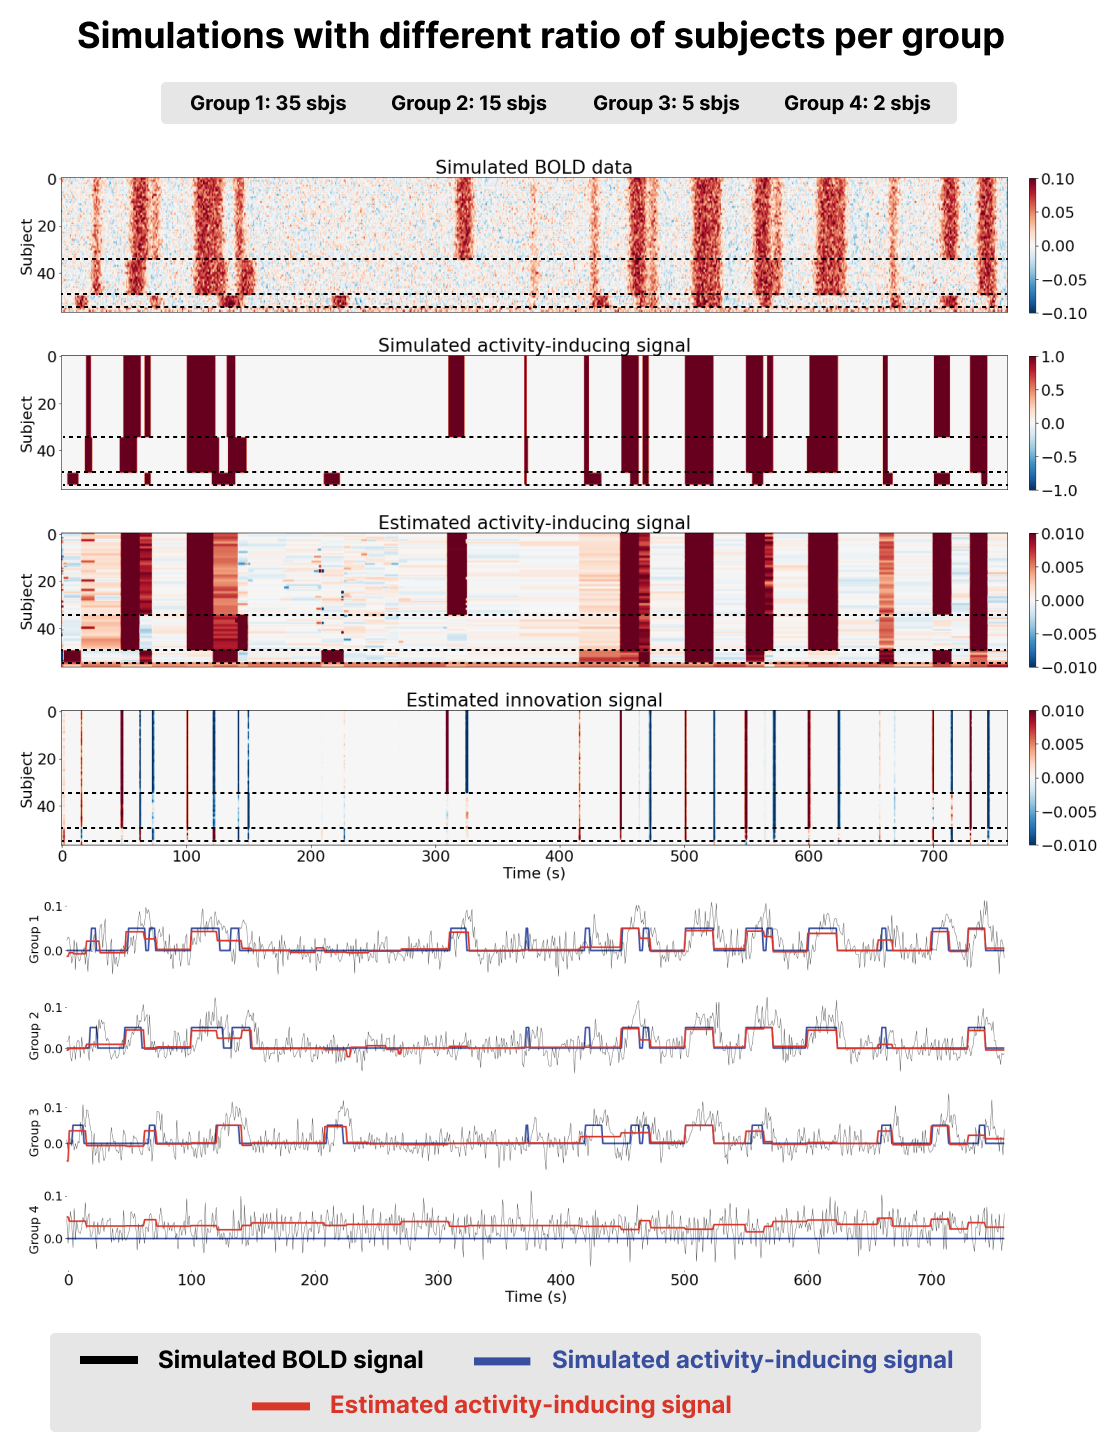
\includegraphics[width=0.8\linewidth]{figures/multi_subject/sim_diff_ratio.png}
    \caption{Results of running msPFM on simulated data for a ratio of subjects
    per group of 35, 15, and 5 subjects respectively (groups are separated by a
    dashed line). The first two heatmaps represent the simulated BOLD and
    activity-inducing signals for all the simulated subjects. The third and
    fourth heatmaps represent the estimated activity-inducing and innovation
    signals for all the simulated subjects. The time courses below depict the
    simulated BOLD (black) and activity-inducing (blue) signals for a subject in
    each group and the estimated activity-inducing signal is shown in red.}
    \label{fig:simulations_diff}
\end{figure}


\begin{figure}[!ht]
    \centering
    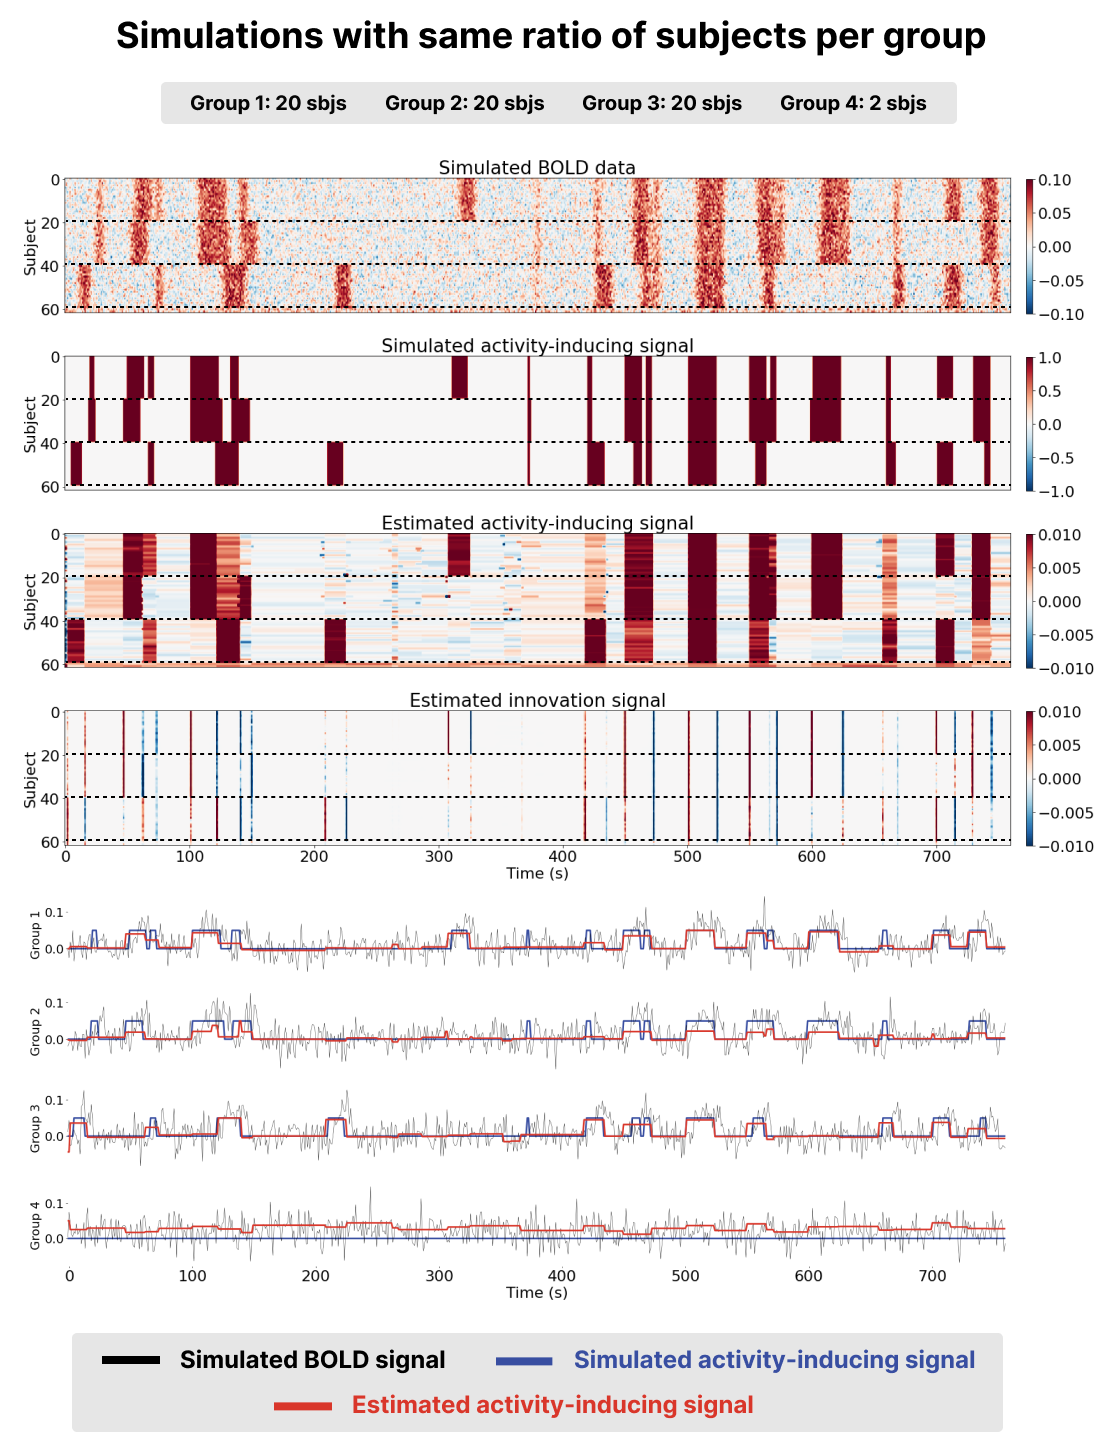
\includegraphics[width=0.8\linewidth]{figures/multi_subject/sim_same_ratio.png}
    \caption{Results of running msPFM on simulated data for a ratio of subjects
    per group of 20, 20, and 20 subjects respectively (groups are separated by a
    dashed line). The first two heatmaps represent the simulated BOLD and
    activity-inducing signals for all the simulated subjects. The third and
    fourth heatmaps represent the estimated activity-inducing and innovation
    signals for all the simulated subjects. The time courses below depict the
    simulated BOLD (black) and activity-inducing (blue) signals for a subject in
    each group and the estimated activity-inducing signal is shown in red.}
    \label{fig:simulations_same}
\end{figure}

Benchmarking msPFM on simulated data where the ground truth is known enables to
assess whether it can effectively identify shared neuronal responses across
subjects, while accommodating individual differences in response to naturalistic
stimuli. The two simulation scenarios described in
\cref{sec:multi_subject_methods} were employed here.

Visual inspection of the results, as presented in the bottom two heatmaps and
the red time courses on \cref{fig:simulations_diff} and
\cref{fig:simulations_same}, revealed that the activity-inducing signal
estimated by msPFM closely resembled the ground truth. This was true for both
scenarios, with an unequal and an equal number of subjects per group. msPFM
demonstrates proficiency in estimating prolonged activity-inducing signals owing
to the adequacy of using a model that estimates the innovations, albeit with
relatively lower accuracy in capturing shorter, transient activations (we refer
the reader to \cite{Urunuela2023HemodynamicDeconvolutionDemystified} for an
in-depth comparison between models based on the activity-inducing signal --the
spike model-- or the innovations --the block model). Furthermore, the influence
of the $\ell_{2,1}$-norm (see \cref{eq:inverse_problem_multi_subject}) is
conspicuous in the estimation of group four, which lacks simulated
activity-signal. In this case, artifacts originating from the estimates of the
remaining groups are noticeable, yet these artifacts are relatively minor
compared to the estimated activity-inducing signals of the other groups. In
addition, the estimated signals for these subjects never return to zero, making
it unlikely that they represent any neuronal-related activity and easily
identifiable as artefacts. These results are consistent for both scenarios.
Hence, based on the simulations, msPFM can pinpoint events that trigger shared
and individualized neuronal responses without knowing their timings.

\subsection{PopSync+ Proof of Concept: Individual and Group Responses to Naturalistic Stimuli}

\begin{figure}[!ht]
\centering
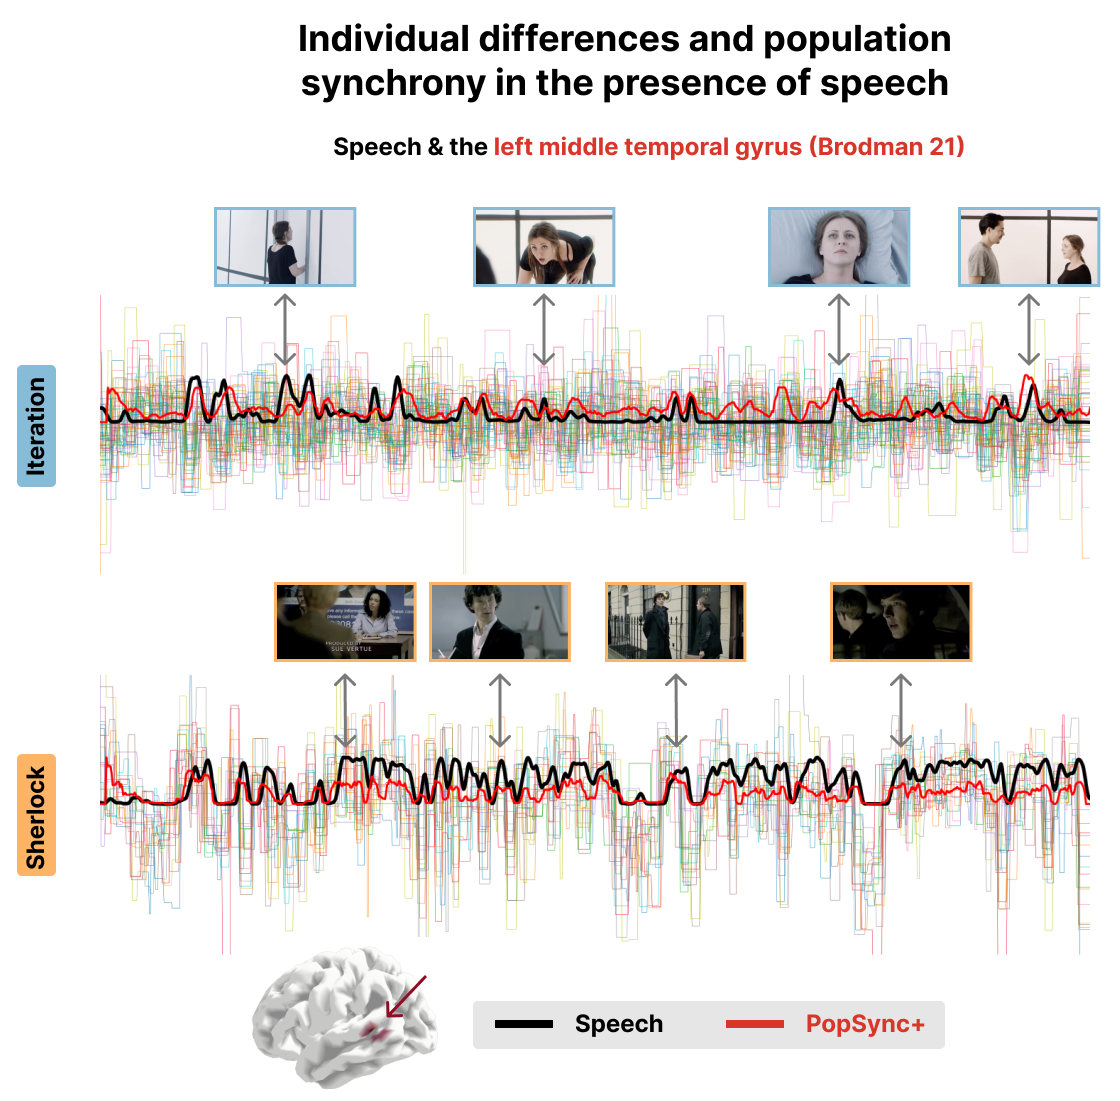
\includegraphics[width=0.9\linewidth]{figures/multi_subject/time_speech.png}
\caption[]{Time series of the estimated activity-inducing signal for each
subject in the left middle temporal gyrus (Brodman 21 area) for the
\textit{Iteration} (top) and \textit{Sherlock} (bottom) datasets. The black
lines represent the speech events in the movie. The red lines represent the
PopSync+, i.e., the sum across subjects of the activity-inducing signal that
evokes a positive BOLD response in each parcel. Representative instances of the
movies and their respective Speech and PopSync+ TRs are shown for both
datasets.}
\label{fig:time_series_speech}
\end{figure}

\begin{figure}[!ht]
\centering
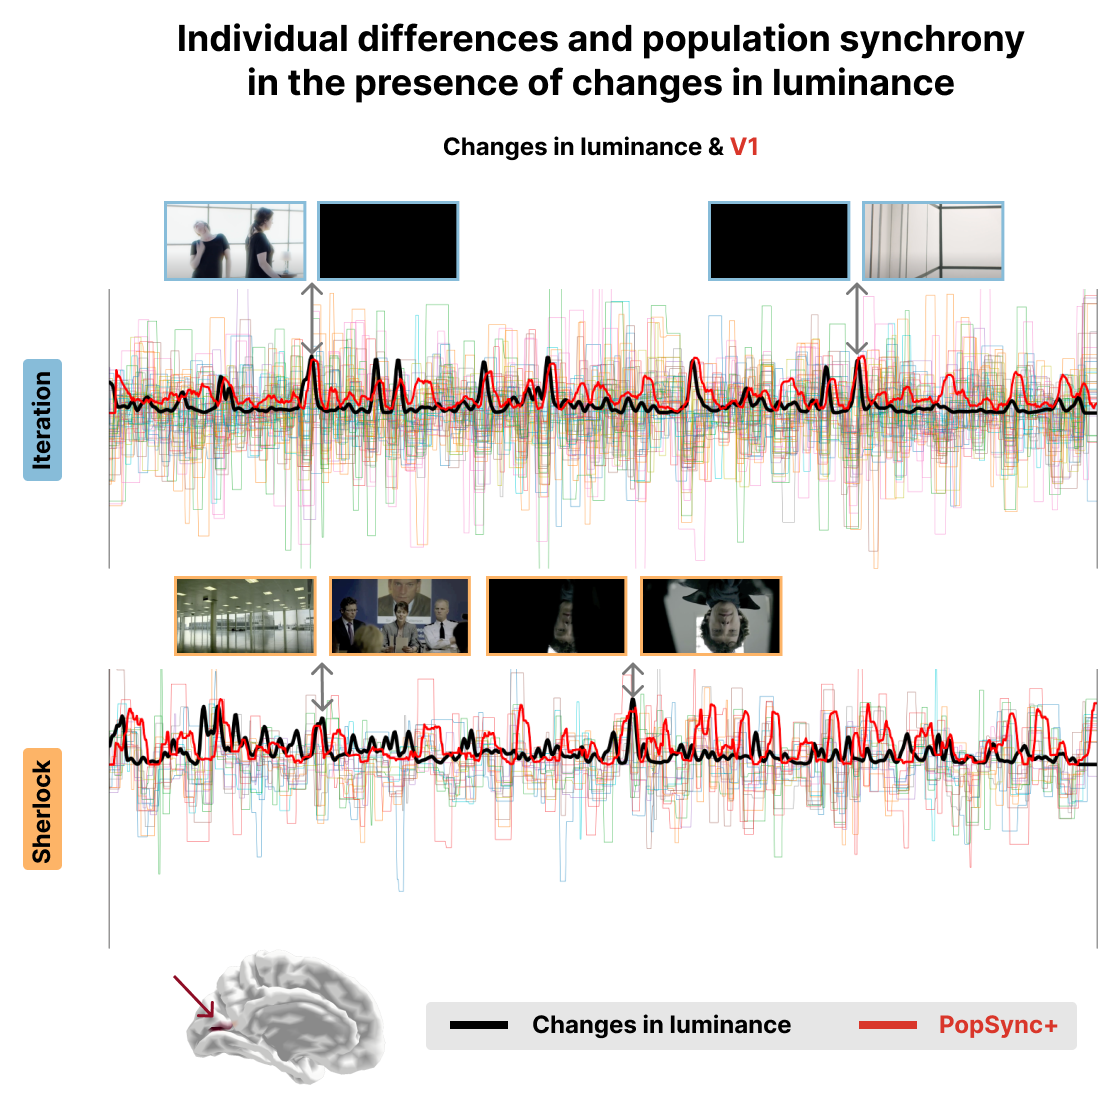
\includegraphics[width=0.9\linewidth]{figures/multi_subject/time_luminance.png}
\caption[]{Time series of the estimated activity-inducing signal for each
subject in V1 for the \textit{Iteration} (top) and \textit{Sherlock} (bottom)
datasets. The black lines represent the changes in luminance in the movie. The
red lines represent the PopSync+, i.e., the sum across subjects of the
activity-inducing signal that evokes a positive BOLD response in each parcel.
Representative instances of the movies and their changes in luminance and
PopSync+ TRs are shown for both datasets.}
\label{fig:time_series_luminance}
\end{figure}

\cref{fig:time_series_speech} and \cref{fig:time_series_luminance} show a proof
of concept of the PopSync+ metrics and the individual differences in the
estimated activity-inducing signal. In fact, the thinner time series in both
datasets clearly demonstrate the presence of individual differences in the msPFM
estimates of each subject, ehich are consistly observed in the two examples of
the left middle temporal gyrus (Brodman area 21) and the V1 visual area.
Notably, the \acrshort*{popsync} time series (depicted in red) displays a
pronounced alignment with speech events occurring in the movies (depicted in
black). This alignment is particularly prominent in the context of
\textit{Sherlock}, wherein the episode encompasses a notably higher frequency of
speech events compared to \textit{Iteration}. In the case of the latter, msPFM
not only captures the speech events but also identifies additional neural
dynamics during non-speech periods in this ROI. \cref{fig:time_series_luminance}
illustrates the synchrony between changes in the luminance of the movies and the
PopSync+ in V1. Specifically, a stronger alignment is observed in the case of
\textit{Iteration}, where the changes in luminance exhibit greater extremes
compared to the case of \textit{Sherlock}, which is also reflected in the
estimated neuronal response in V1 and hence the PopSync+ measure.

\subsection{Comparison with Hidden Markov Models and Inter-Subject Correlation}

\begin{figure}[!ht]
\centering
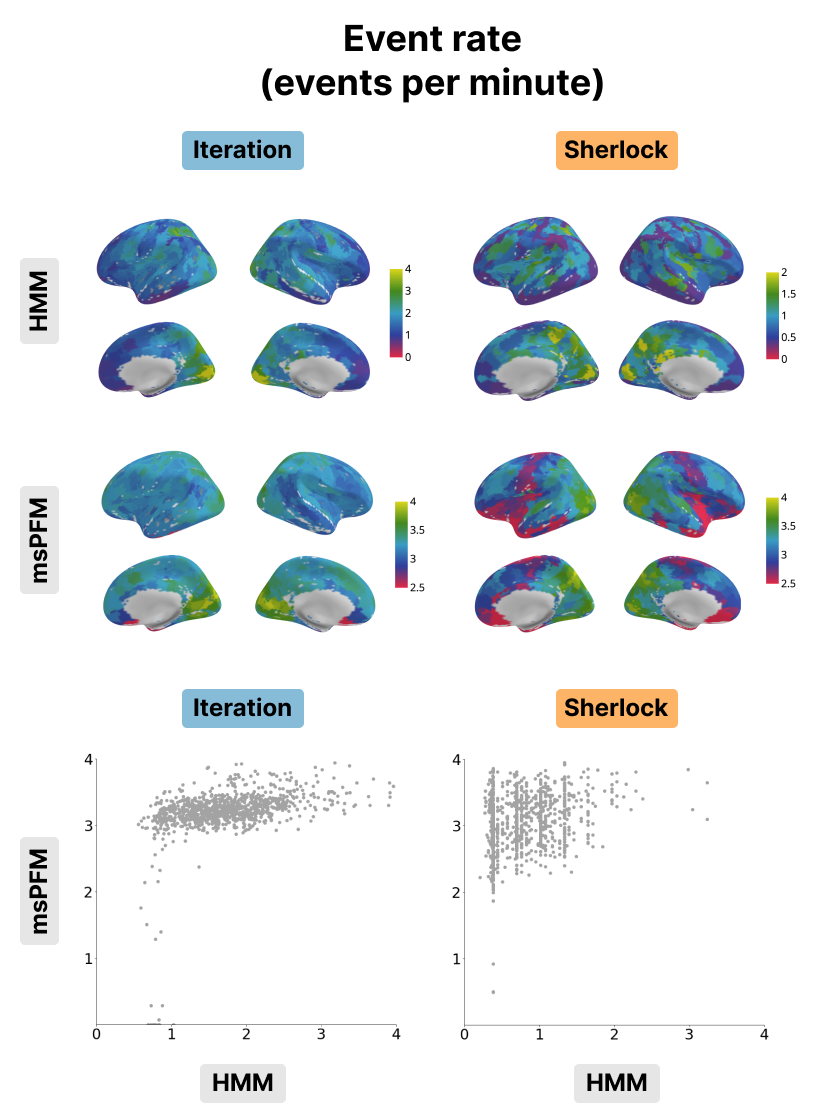
\includegraphics[width=0.7\linewidth]{figures/multi_subject/event_rate.png}
\caption[]{Event rate for the \textit{Iteration} (left) and \textit{Sherlock}
(right) datasets. The event rate maps obtained with the HMM (top) and msPFM
algorithms (bottom) are compared. The bottom row shows the differences in values
between msPFM and the HMM approach.}
\label{fig:event_rate}
\end{figure}

\begin{figure}[!ht]
\centering
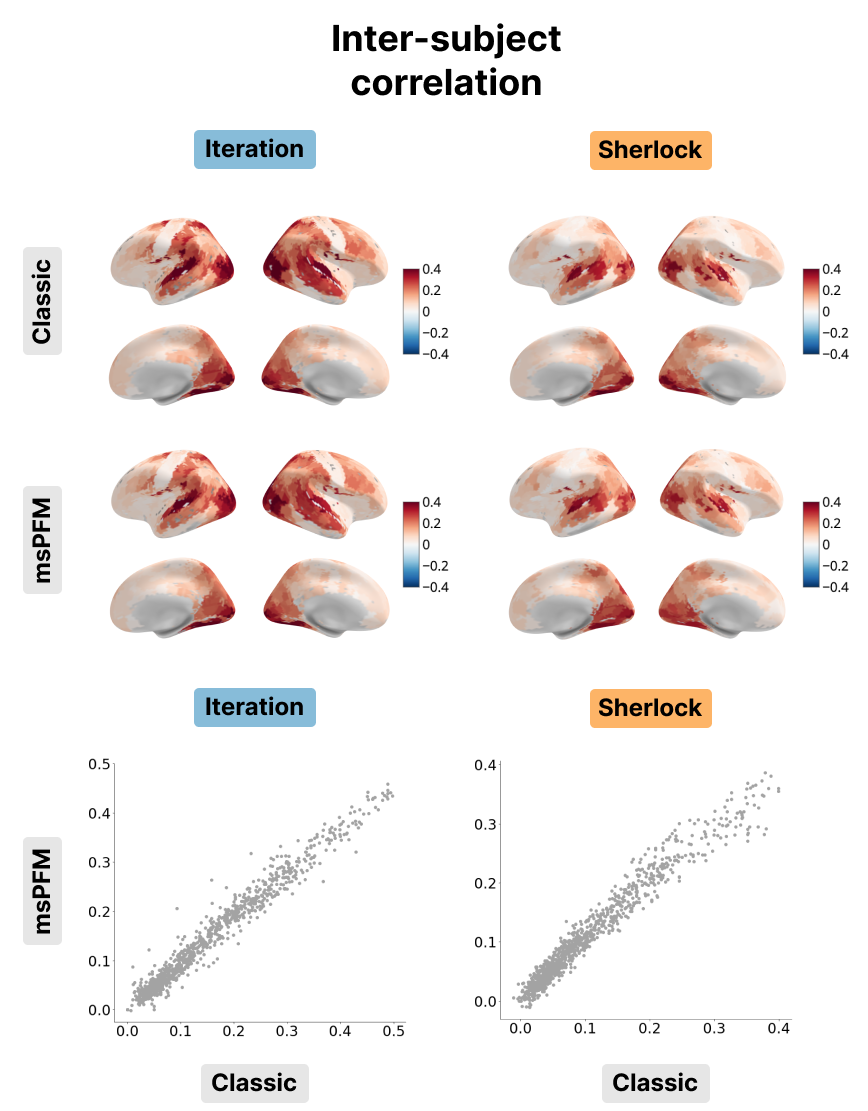
\includegraphics[width=0.7\linewidth]{figures/multi_subject/inter_subject.png}
\caption[]{Inter-subject correlation for the \textit{Iteration} (left) and
\textit{Sherlock} (right) datasets. The inter-subject correlation obtained with
msPFM (bottom) is compared with the inter-subject correlation obtained with the
classic approach (top). The bottom row shows the differences in values between
msPFM and the classical ISC approach.}
\label{fig:isc}
\end{figure}

As shown in \cref{fig:event_rate}, the event rates of both HMM and msPFM for the
\textit{Iteration} dataset show a posterior-to-anterior cortical gradient with a
higher frequency of events in posterior, sensory regions and slower rates in
anterior, higher-order regions. This gradient is consistent with previous
findings in the literature \citep{SavaSegal2022Individualvariabilityneural}.
However, the scatter plots in the bottom row illustrate that the difference in
event rates between posterior and anterior regions is less pronounced in the
case of msPFM as compared with the HMM. This discrepancy can be attributed to
the divergent definitions of what an event is for the two methods. The HMM
approach identifies states that are expected to persist for a specific number of
time points, while the msPFM algorithm captures "punctate" events that can be
directly associated with individual moments in the stimulus. As a consequence,
the msPFM algorithm is expected to detect a greater number of events,
particularly in anterior regions. In the context of the \textit{Sherlock}
dataset, it is worth noting that the event rate is noticeably lower when
calculated with HMM, and consequently, the cortical gradient is less apparent.
On the other hand, the msPFM event rate demonstrates values similar to
\textit{Iteration} and reveals a more distinct cortical gradient. When it comes
to the inter-subject correlation, the two maps and their values were remarkably
similar as shown in \cref{fig:isc}, indicating that msPFM is able to recover
this same sensory-association gradient, with subjects being more synchronized
with one another lower-order regions, while being more idiosyncratic in
higher-order regions.

\subsection{Benchmark Against Low- and Mid-Level Movie Features}

\begin{figure}[!ht]
    \centering
    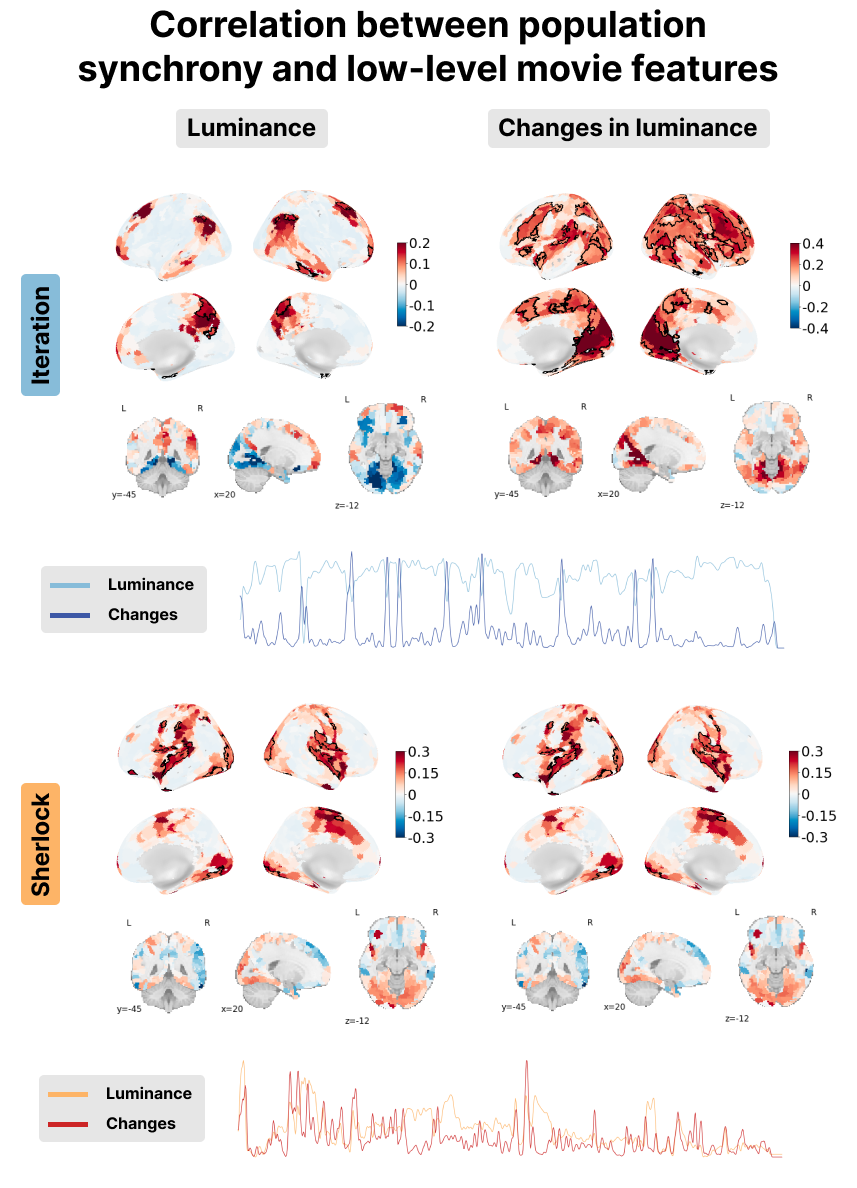
\includegraphics[width=0.7\linewidth]{figures/multi_subject/low_order_luminance.png}
    \caption[]{Correlation between the PopSync+ and low-level features of the
    movie with luminance on the left and its derivative on the right.
    Significant regions are highlighted by a black contour, while
    non-significant regions are displayed with increasing transparency as the
    correlation values are further from the significance threshold. The
    correlation maps are shown for the \textit{Iteration} (top) and
    \textit{Sherlock} (bottom) datasets. The time courses below depict the
    luminance (lighter color) and its derivate (darker color) for
    \textit{Iteration} (blue) and \textit{Sherlock} (red).}
    \label{fig:low_order_luminance}
\end{figure}

\begin{figure}[!ht]
    \centering
    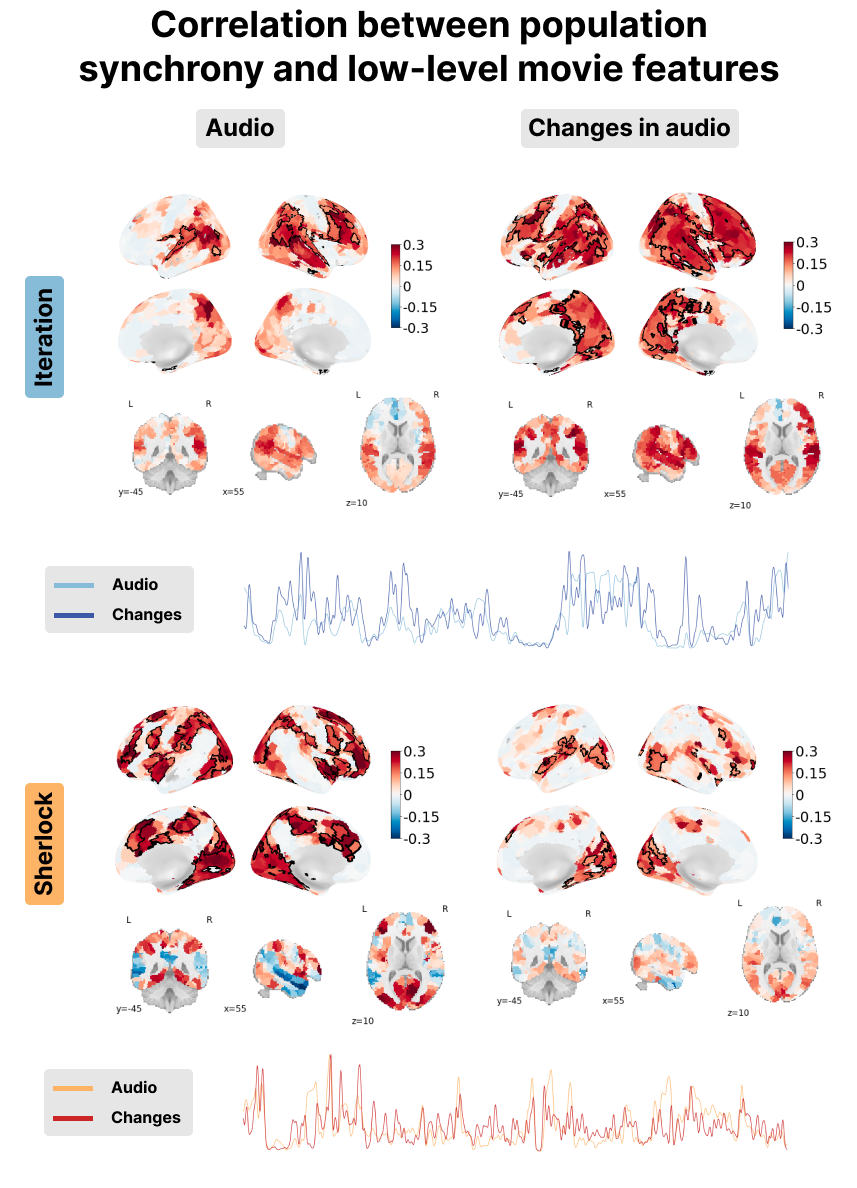
\includegraphics[width=0.7\linewidth]{figures/multi_subject/low_order_audio.png}
    \caption[]{Correlation between the PopSync+ and low-level features of the
    movie with luminance and its derivative on the left, and the audio envelope
    and its derivative on the right. Significant regions are highlighted by a
    black contour, while non-significant regions are displayed with increasing
    transparency as the correlation values are further from the significance
    threshold. The correlation maps are shown for the \textit{Iteration} (top)
    and \textit{Sherlock} (bottom) datasets. The time courses of the audio
    envelope (lighter color) and its derivate (darker color) are shown in blue
    for \textit{Iteration} and in red for \textit{Sherlock}.}
    \label{fig:low_order_audio}
\end{figure}

The results of the correlation analysis with the low- and mid-level movie
features are shown in \cref{fig:low_order_luminance},
\cref{fig:low_order_audio}, \cref{fig:mid_order_speech_hands} and
\cref{fig:mid_order_faces} respectively.

In terms of luminance, our observations reveal contrasting patterns between
\textit{Sherlock} and \textit{Iteration} in regions of the visual cortex. While
\textit{Sherlock} demonstrates a positive correlation, indicating a relationship
between luminance and brain activity, \textit{Iteration} exhibits a negative
correlation in the same regions. Conversely, when examining changes in luminance
(i.e., the derivative of the luminance time course), both datasets display a
positive correlation within the visual cortex. These findings can be interpreted
as a consequence of the luminance adaptation in \textit{Iteration}. The movie
predominantly features very bright scenes, occasionally transitioning to dark
moments as shown in the blue time courses at the bottom left of
\cref{fig:low_order_luminance}. In contrast, \textit{Sherlock} contains more
diverse scenes in multiple locations, thereby exhibiting a greater range of
luminance with both the luminance and its derivative being very similar (see red
time courses in the bottom left of \cref{fig:low_order_luminance}).

The audio envelope analysis reveals a noteworthy positive correlation within
regions of the auditory cortex for both datasets, with a more pronounced
correlation observed in \textit{Iteration}. Examination of audio envelope
variations, i.e., the derivate of the audio envelope, further demonstrates a
robust positive correlation within the auditory cortex for both datasets. In
this case, both the audio envelope and its derivate showed a very similar
pattern (see red and blue time courses in the bottom right of
\cref{fig:low_order_audio}). This underscores the ability of msPFM to accurately
capture the intricate neural dynamics associated with the auditory component of
the movies.

\begin{figure}[!ht]
\centering
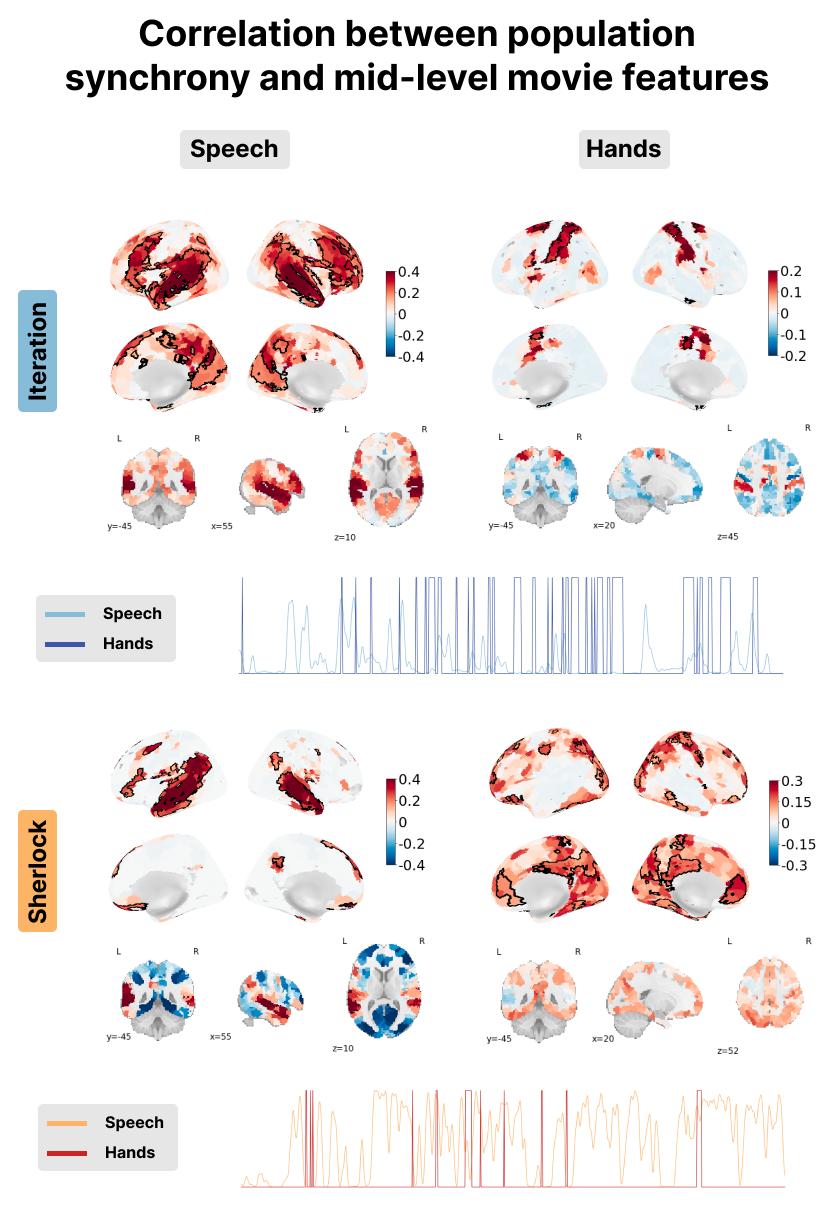
\includegraphics[width=0.7\linewidth]{figures/multi_subject/mid_order_speech_hands.png}
\caption[]{Correlation between the PopSync+ and mid-level features of the movie
with the presence of speech on the left and hands on the right. Significant
regions are highlighted by a black contour, while non-significant regions are
displayed with increasing transparency as the correlation values are further
from the significance threshold. The correlation maps are shown for the
\textit{Iteration} (top) and \textit{Sherlock} (bottom) datasets. The time
courses below depict the presence of speech (lighter color) and hands (darker
color) for \textit{Iteration} in blue and \textit{Sherlock} in red.}
\label{fig:mid_order_speech_hands}
\end{figure}

\begin{figure}[!ht]
\centering
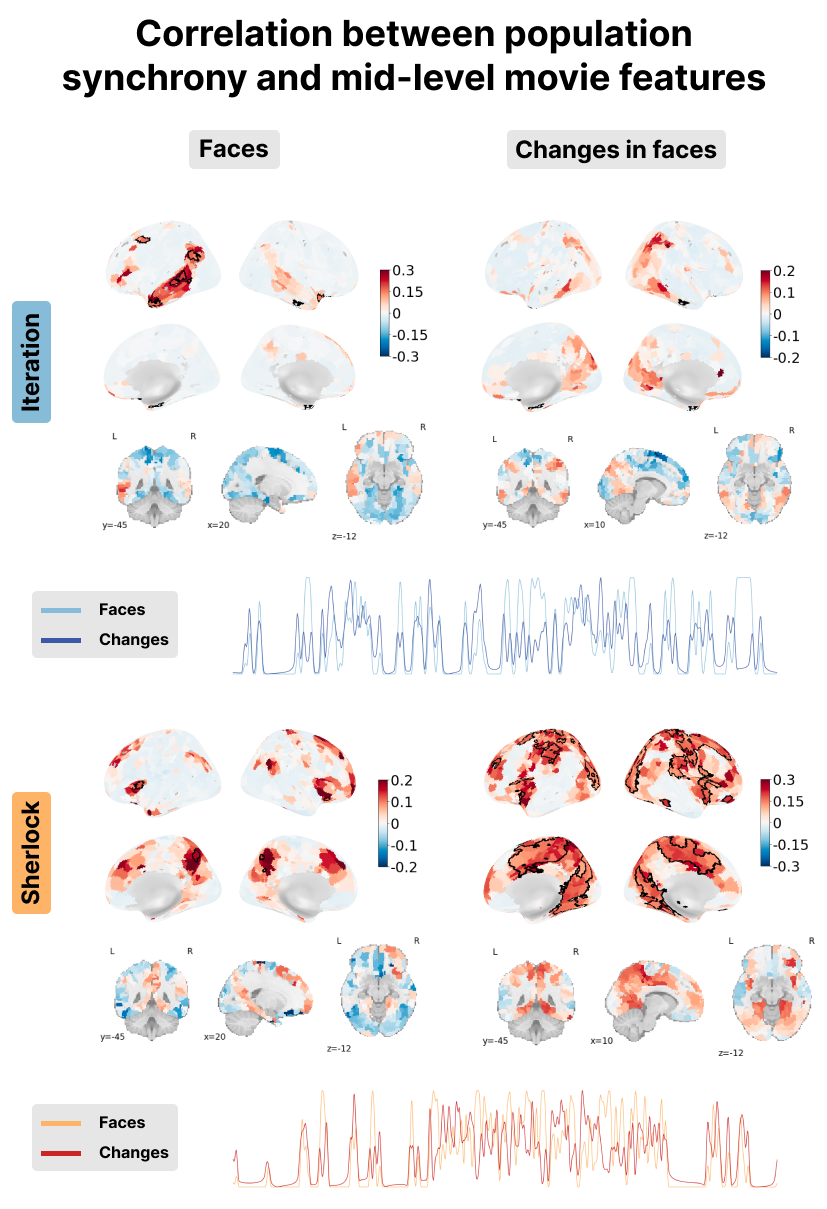
\includegraphics[width=0.7\linewidth]{figures/multi_subject/mid_order_faces.png}
\caption[]{Correlation between the PopSync+ and mid-level features of the movie
with the presence of faces on the left and its derivative on the right.
Significant regions are highlighted by a black contour, while non-significant
regions are displayed with increasing transparency as the correlation values are
further from the significance threshold. The correlation maps are shown for the
\textit{Iteration} (top) and \textit{Sherlock} (bottom) datasets. The time
courses of the presence of faces (lighter color) and its derivate (darker color)
are shown in blue for \textit{Iteration} and red for \textit{Sherlock}.}
\label{fig:mid_order_faces}
\end{figure}

Next, mid-level movie features were examined, including the presence of speech
as well as hands and faces onscreen. Significantly, it can be observed that
msPFM adeptly captures the intricate neural dynamics linked to speech in both
datasets, revealing large correlations in expected areas of the superior
temporal gyrus, Heschl's gyrus, middle temporal and inferior frontal gyrus, all
of them bilaterally. These maps demonstrate the adaptability of msPFM to capture
varying amounts of speech present in the respective movies. This adaptability is
particularly pronounced in the context of \textit{Iteration}, characterized by a
scarcity of speech compared to \textit{Sherlock}---a movie abundant in speech-
as shown in the time courses in the bottom left of
\cref{fig:mid_order_speech_hands}. Notwithstanding this discrepancy, msPFM
reliably captures the neural dynamics associated with speech in language-related
areas, reaffirming its efficacy. 

Furthermore, positive correlation between the msPFM-estimated activity-inducing
signal and the presence of hands in the movies can also be observed in bilateral
sensorimotor regions around the central sulcus. In the context of
\textit{Iteration}, the correlation was observed prominently within regions of
the somatosensory cortex (i.e. postcentral gyrus) and supplementary motor areas,
while \textit{Sherlock} exhibited correlation within more anterior regions in
the motor cortex (i.e. precentral gyri). These findings could potentially be
explained by the contrasting composition of \textit{Iteration} and
\textit{Sherlock}. While \textit{Iteration} predominantly incorporates hands in
relation to other objects or the main character's actions (see the high
frequency in the blue time course at the bottom left of
\cref{fig:mid_order_speech_hands}), it features fewer hands-only shots. On the
other hand, \textit{Sherlock} exhibits a higher frequency of hands-only shots
(though few across the entire movie as shown in red in the bottom left time
course in \cref{fig:mid_order_speech_hands}), which may account for the
aforementioned findings.

Finally, as shown in \cref{fig:mid_order_faces}, correlation between the
PopSync+ time-series and the presence of faces was found in the
\textit{Iteration} movie in the left middle temporal gyrus, a region associated
with facial familiarity \citep{Zhen2013HierarchicalBrainNetwork}, and the
posterior superior temporal sulcus, a region associated with the processing of
gaze and expression \citep{Baseler2012NeuralResponsesExpression}. This finding
aligns with the movie's nature, as \textit{Iteration} predominantly features a
single character and contains several headshots where viewers have their eyes
locked on the character's eyes and can see her facial expression. No significant
or substantial correlation between the PopSync+ measure and the presence of
faces was found in the movie in the \textit{Sherlock} dataset. However, when
focusing on changes in faces specifically within the \textit{Sherlock} dataset,
a positive correlation was observed in the fusiform gyrus, a region associated
with face recognition
\citep{Kanwisher1997FusiformFaceArea,Kanwisher2006fusiformfacearea,Rossion2003functionallydefinedright}
Interestingly, this correlation with changes in faces was not as strong when
examining changes in faces for \textit{Iteration}. These contrasting findings
may be attributed to the distinctive characteristics of the movies. In
\textit{Sherlock}, which showcases multiple characters and their facial
expressions during dialogue, the adaptation or identification of faces may play
a role (see long periods of changing faces in the red time courses at the bottom
of \cref{fig:mid_order_faces}). On the contrary, \textit{Iteration} primarily
focuses on a single character, suggesting an fMRI adaptation effect in fusiform
face areas, i.e. a lower response to an identically repeated face than to new
faces
\citep{Gauthier2001developmentfaceexpertise,Yovel2004FacePerception,Avidan2010Corticalnetworksmediating,Eger2005Familiarityenhancesinvariance,Pourtois2005Twoelectrophysiologicalstages,Rotshtein2004MorphingMarilynMaggie}.

Overall, these analyses showcase the potential of msPFM in capturing the
activity linked to lower- and mid-level stimulus features within anticipated
brain regions and timeframes, even without prior knowledge of event timings and
regardless of the stimulus itself. Furthermore, these findings highlight the
ability of msPFM to identify additional stimulus-specific regions associated
with the intricate and distinctive content inherent to each stimulus.

\section{Discussion}
\label{sec:multi_subject_discussion}

The potential of multi-subject \acrlong*{pfm} (msPFM) to detect and elucidate
moment-to-moment spatio-temporal neural activity patterns evoked by naturalistic
stimuli has been showcased using simulations and two experimental datasets.
While previous investigations have employed alternative approaches, such as
hidden Markov models (HMM) \citep{Baldassano2017DiscoveringEventStructure},
greedy state boundary search (GSBS) \citep{Geerligs2021Detectingneuralstate},
inter-subject correlation \citep{Nastase2019Measuringsharedresponses} or dynamic
functional connectivity \citep{Di2020Intersubjectconsistentdynamic}, these
methods operate on a limited number of regions of interest (ROIs) and condense
the temporal dynamics of the BOLD signal into states or connectivity patterns
that encompass a time period exceeding the acquired data's temporal resolution.
Consequently, the results shown here highlight the unparalleled potential of
msPFM to operate at the utmost temporal and spatial precision achievable.

Importantly, msPFM was validated by comparing it against other common algorithms
used to assess naturalistic fMRI data, such as Hidden Markov Models (HMM) and
intersubject correlation (ISC). First, the event-rate analysis shown in
\cref{fig:event_rate} revealed a distinct cortical gradient, characterized by
faster event rates in posterior sensory regions and slower rates in anterior
higher-order regions. These results align with previous findings on neural event
boundaries across subjects and the segmentation of events using HMM
\citep{Baldassano2017DiscoveringEventStructure,SavaSegal2022Individualvariabilityneural},
which could support the idea that the brain's cortical organization is arranged
hierarchically, with sensory inputs passing through unimodal areas and being
abstracted into broader conceptual and cognitive representations in transmodal
areas
\citep{Bernhardt2022Gradientsbrainorganization,Margulies2016Situatingdefaultmode,Samara2023Corticalgradientsnaturalistic}.
However, msPFM offers several advantages over the HMM-based approach. First, the
\acrshort*{hmm} method requires specifying a desired number of events ($k$) for
each region. While there are data-driven ways to estimate an appropriate value
for $k$ at the group level, these require additional computational time and
power, and are not straightforward to implement for individual subjects. In
contrast, msPFM does not require pre-specifying any value of $k$, and instead
recovers individual neuronal-related events at both the group and individual
level. Furthermore, the HMM model assumes that each "state" exhibits a unique
neural activity signature that changes at state boundaries, which may not hold
true universally, as certain brain regions could potentially revert to previous
or new states inside this perdiod. In contrast, msPFM applies no restriction on
the number and duration of the neural activity patterns that can be detected,
thereby providing a more comprehensive representation of the brain's
spatio-temporal dynamics. The crucial distinction is that the HMM approach
identifies events or states that persist for a specific duration, whereas the
msPFM technique retrieves discrete instances of neuronal-related BOLD activity,
which can be directly associated with individual moments in the stimulus.
Another important distinction is the computational cost needed to analyse data
with each of the two techniques. In fact, while finding the appropiate number of
events with HMM can take $>24$h at the single-subject level with 1000 ROIs using
a high performance computing server with up to 512GB of RAM available, finding
estimates of the activity-inducing signal and counting the number of events with
msPFM only took between 5 and 10 minutes.

Furthermore, techniques like HMM and inter-subject correlation are not
specifically designed to detect activity evoked by the stimulus in different
brain regions, but rather to identify regions that encode stimulus-related
information consistently across multiple individuals
\citep{Nastase2019Measuringsharedresponses}. In contrast, msPFM can detect
moment-to-moment neuronal resonses not only shared across subject, but also
distinguish patterns occurring in individual subjects. By correlating the
recovered population synchrony with features of the movies,
\cref{fig:lower_order_correlations} and \cref{fig:higher_order_correlations}
show that msPFM is able to detect neuronal activity driven by both low- and
mid-level features of the stimulus in both primary sensory and higher-order
brain regions. Particularly, fMRI adaptation to the stimulus
\citep{GrillSpector2001fMRadaptationtool} may be present in some features such
as luminance, with the visual cortex mostly showing activity in response to
changes in the luminance in \textit{Iteration} probably due to the increased
contrast associated with these changes
\citep{Goodyear1998EffectLuminanceContrast}; or the presence of faces, with
\textit{Iteration} having a single character and no reliable face-related
activity in the fusiform gyrus as opposed to \textit{Sherlock} and the many
characters in the clip, where the fusiform gyrus showed correlation with changes
in faces
\citep{Kanwisher1997FusiformFaceArea,Kanwisher2006fusiformfacearea,Rossion2003functionallydefinedright}.
The case of \textit{Sherlock} is particularly challenging because faces are
always closely followed by speech, which is a stronger effect and can hide the
response to the presence of faces \citep{Vega2022Neuroscoutunifiedplatform}.

While this study introduces a novel approach for analyzing naturalistic fMRI
data, there is potential for further enhancements. Adopting a data-driven
strategy like stability selection
\citep{Meinshausen2010Stabilityselection, Urunuela2022Wholebrainmultivariate}
could eliminate the need for manually selecting the regularization parameter. By
adopting such an approach, not only would the method's robustness be enhanced,
but it would also enable estimation of the probability of neuronal-related
events at each TR, subject, and voxel or ROI. Additionally, the utilization of
optimal transport methods could further refine the spatial differentiation of
shared and individualized patterns by improving its robustness against
anatomical (spatial) and hemodynamic (temporal) variability between subjects
\citep{Janati2020MultisubjectMEG/EEG}. Nevertheless, the current methodology
adequately demonstrates the potential of msPFM-alike approaches in investigating
the brain's spatio-temporal dynamics during naturalistic stimuli. For instance,
msPFM offers a valuable approach to unraveling the precise neural mechanisms
involved in event segmentation. It can be employed independently or in
conjunction with other techniques such as HMM or \acrshort*{gsbs} to gain an
understanding of the timescale for memory encoding, as well as the continuous
updating or encoding of memory fragments following the completion of an event
\citep{Baldassano2017DiscoveringEventStructure,
Silva2019RapidMemoryReactivation}. Moreover, novel research utilizing msPFM
could be aimed at comprehending how the human brain comprehends these complex
multiplexed signals and understanding the specific features of the stimulus that
elicit responses in the human brain. Finally, the proposed method has the
potential to elucidate the connection between individual differences in these
responses and subsequent memory formation or appraisal of the stimulus.

\section{Code and data availability}
\label{sec:multi_subject_github}
The code and materials used to generate the figures in this work can be found in the following
GitHub repository:
\url{https://github.com/eurunuela/msPFM\_paper}.

The \textit{msPFM} Python package is available in the following GitHub repository:
\url{https://github.com/ParadigmFreeMapping/msPFM}
